\section{Verification overview}%
\label{sec:txn:overview}

\begin{figure}
  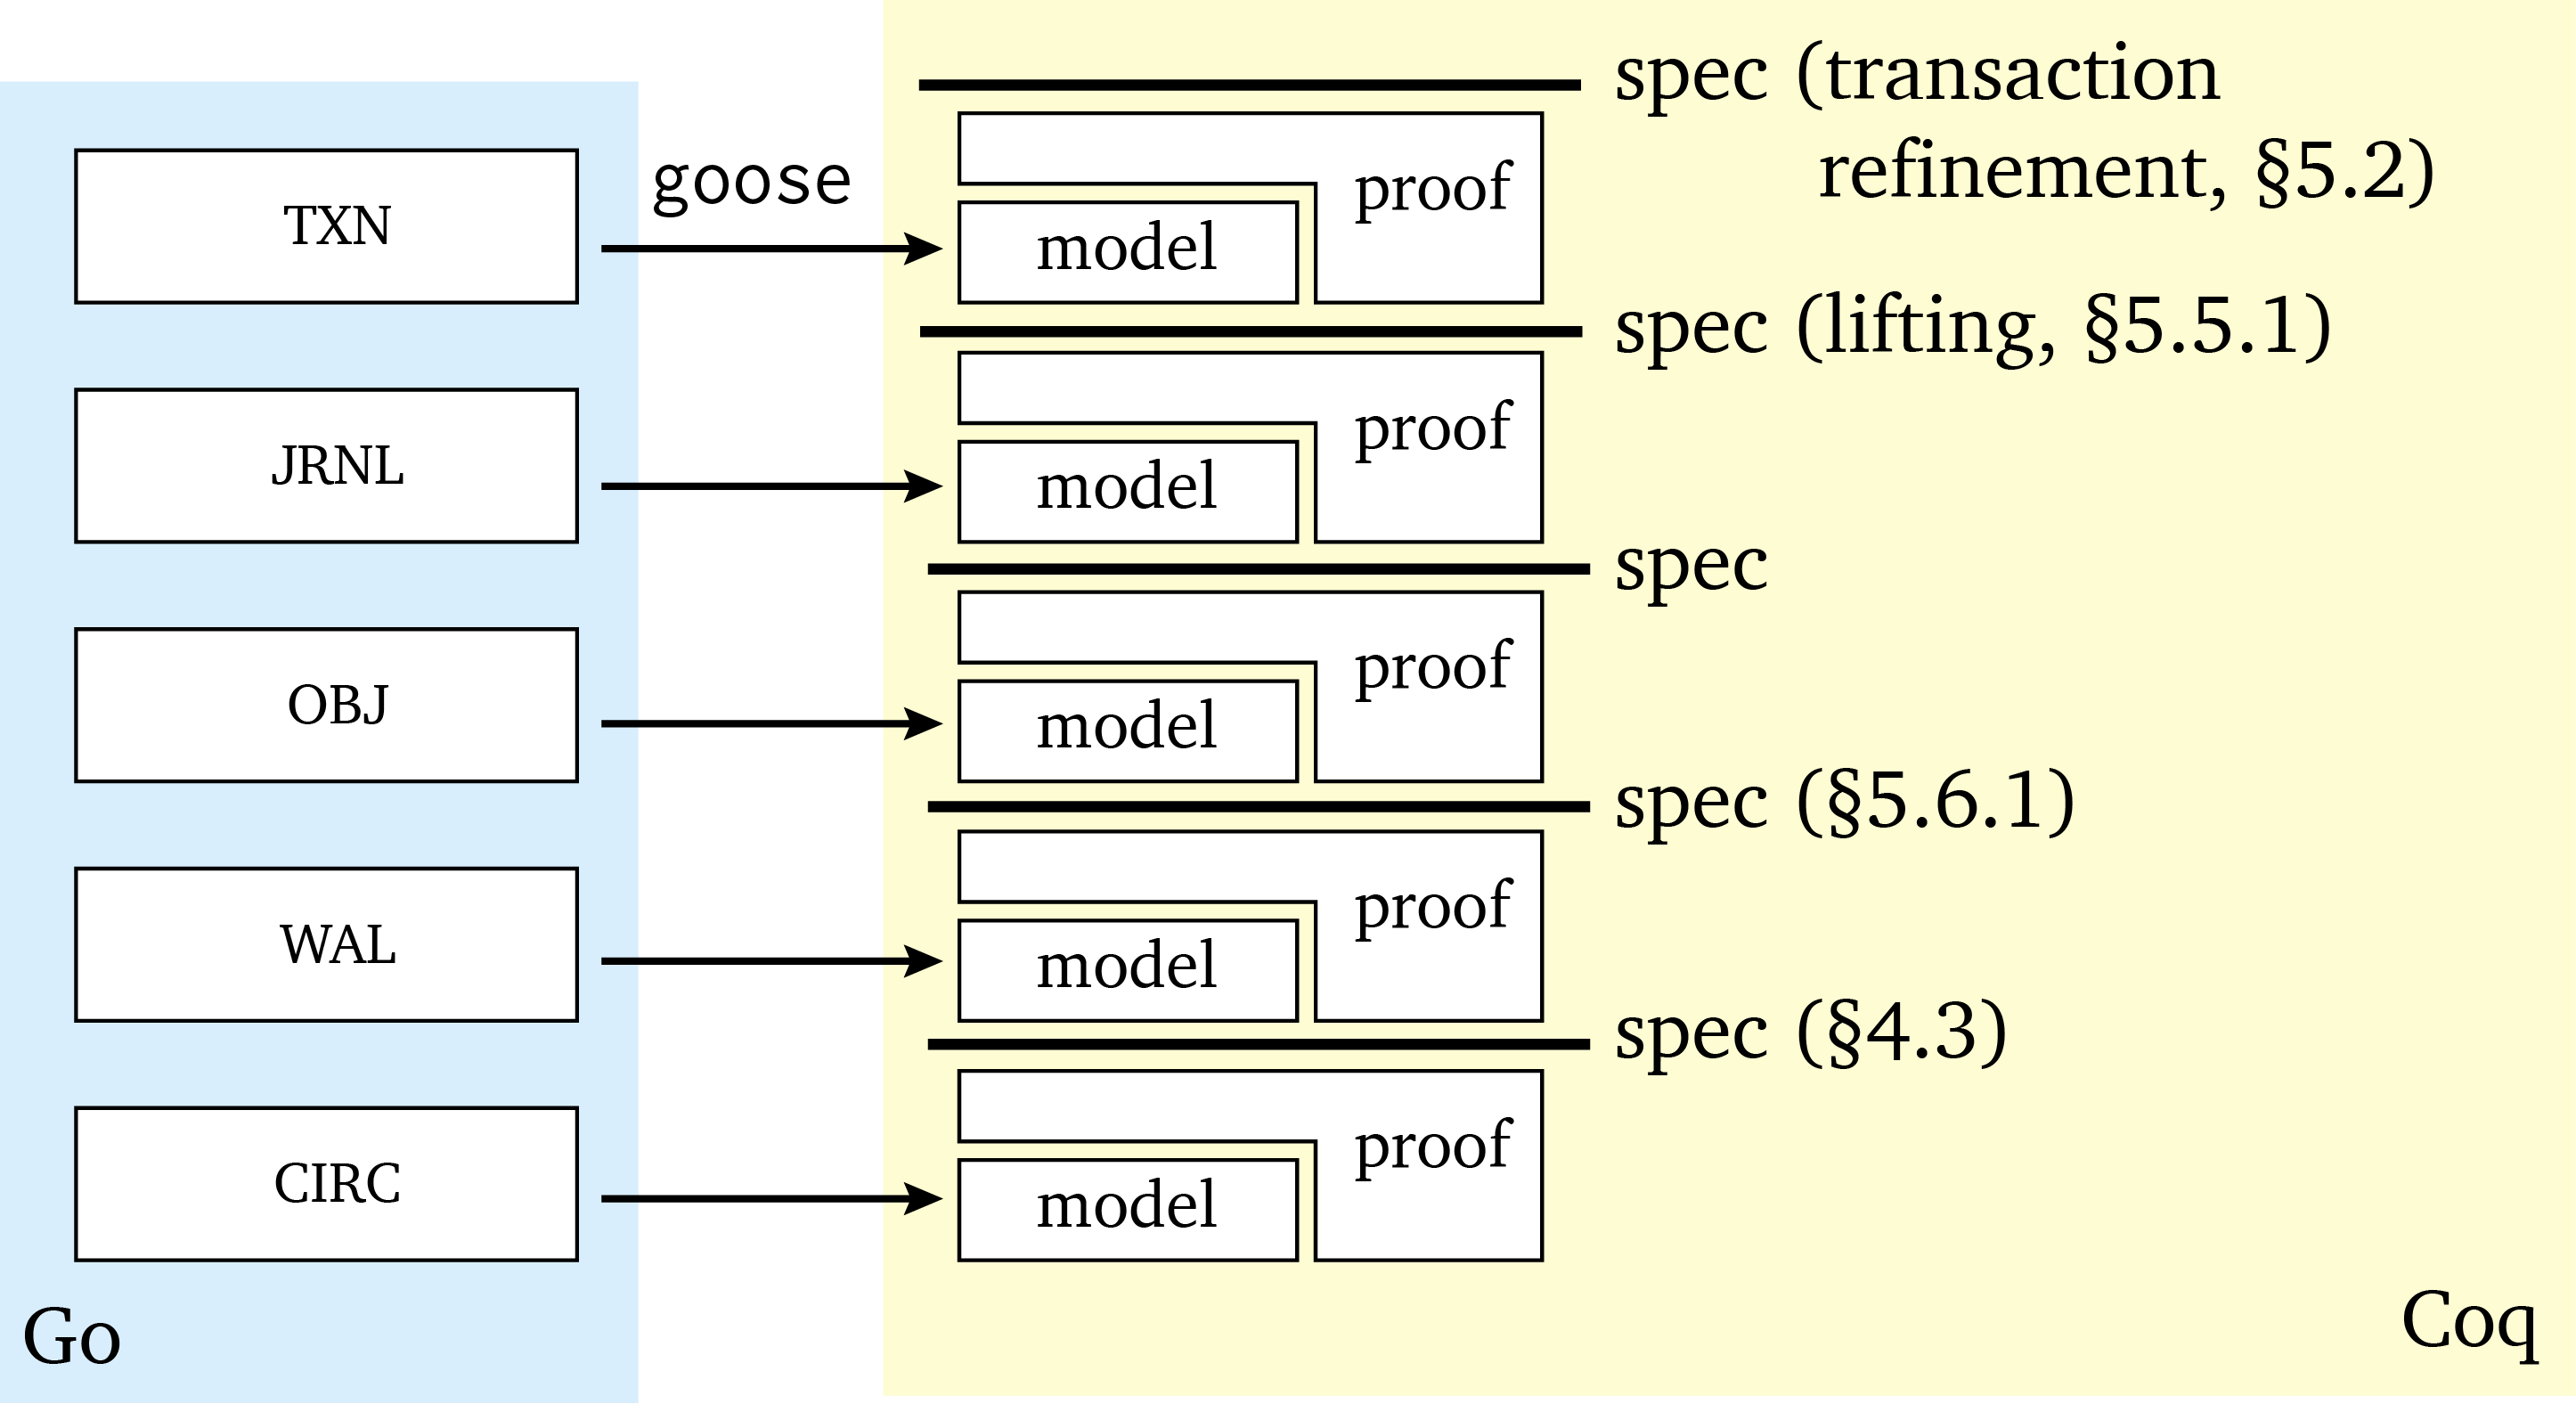
\includegraphics{fig/gotxn.png}
  \caption{Overview of the GoTxn proof, which is divided into proofs for each
    layer. The proofs are all built on top of Perennial.}
  \label{fig:txn:proof-overview}
\end{figure}

\Cref{fig:txn:proof-overview} gives an overview of the libraries (or layers) in
the GoTxn proof. On the left side of the figure is the code, organized into a
stack of libraries, each of which uses the library below. The code is written in
Go and then translated to a model in Coq using Goose (described in
\cref{ch:goose}); each proof is about the model of that library. Each
intermediate layer has a specification which is formally described using
Perennial's logically atomic crash specifications (\scc{txn} has a different
specification). The proofs are all implemented using Perennial for crash safety
and concurrency reasoning, combined with Goose's reasoning principles for Go.

At the bottom level, the \scc{circ} library is implemented using Go primitives
supported by Goose, including an API to access the disk. The disk supports
synchronous reads and writes of 4KB sectors, a standard feature for disk
hardware. On crash, the model of the disk in Perennial assumes writes are atomic
at this 4KB granularity.

At the top level, \scc{txn}'s specification is the program refinement
specification described earlier in \cref{sec:txn:spec}. This specification is
about an arbitrary program that uses GoTxn, which is formalized using GooseLang,
the language that we use to model Go code. Note that the statement of program
refinement only talks about the GoTxn implementation and a (GooseLang) program
using it; it no longer references the Perennial logic. We are able to prove such
a theorem because Perennial comes with a soundness theorem that relates the
theorems proven using Perennial's crash specifications to the code's execution.
Making the final theorem independent of the logic is important in the next
chapter, \cref{ch:daisy-nfs}, which connects the GoTxn specification to proofs
in Dafny that do not use the Perennial logic.
